\section{Grundlagen}
\label{sec:3}
Dieses Kapitel umfasst die technischen Grundlagen, auf denen diese Arbeit aufbaut. 
Es wird ein Einblick in die Funktionsweise von VR gegeben, um das Problem bisheriger Lösungen 
besser zu verstehen. Außerdem werden bewährte Methoden zur Feuer- und Rauchsimulation
gesammelt und erklärt. Ein weiterer Teil dieses Kapitels setzt sich mit grundlegendem Texture Mapping,
Bump- und Displacement Mapping, sowie Parallax- und Parallax Occlusion Mapping auseinander. Abschließend 
werden noch zwei Volume Rendering-Methoden vorgestellt: Ray Marching und Texturbasiertes Volume Rendering.

\subsection{Virtual Reality}
\subsubsection{Konzept}

Hinter dem Begriff Virtual Reality (VR) verbirgt sich das Konzept einer
künstlichen, von Computern generierten Welt.
Der Nutzer kann in diese Welt eintauchen und hat dabei die Möglichkeit, sich als Betrachter in dieser Welt
umzuschauen, oder sogar mit dieser Welt zu interagieren. Das erste Konzept eines VR-Headsets mit Kopftracking
wurde bereits in den 60er Jahren von Ivan Sutherland entworfen. \parencite{Sutherland1965, Sutherland1968}

Heutzutage gibt es verschiedene Arten von VR. Zum einen die "Non-immersive Virtual Reality".
Hierbei steuert der Nutzer seine virtuelle Umgebung, ist sich dabei aber noch bewusst,
in welcher Realität er sich tatsächlich befindet. Die Interaktion geschieht üblicherweise durch
Eingabegeräte wie Controller, Maus oder Tastatur. Ein weit verbreitetes Anwendungsgebiet sind
dabei herkömmliche Videospiele. Gegenüberstehend gibt es dagegen die "Fully Immersive Virtual Reality".
Hierbei wird der Nutzer durch spezielle Hardware, zum Beispiel mithilfe eines Head-Mounted-Displays (HMD),
einem sogenannten VR-Headset, selbst in eine virtuelle dreidimensionale Umgebung versetzt.
Durch visuelles, auditives und teilweise auch haptisches Feedback kann der Nutzer dabei immer weiter
in die virtuelle Welt eintauchen.
Auch hier verfügt der Nutzer über spezielle Eingabegeräte wie dem Headset, Controllern oder Laufbändern. Diese sind
jedoch in ihrer Benutzung näher an der bekannten Realität. So kann sich der Nutzer z.B. mit einer Kopfbewegung
in der virtuellen Welt umsehen oder Dinge anfassen und mit diesen interagieren. Dieser Einfluss auf die
Umgebung sorgt dafür, dass sich eine Simulation echter anfühlen kann.

Die Idee von Fully Immersive Virtual Realities baut dabei darauf auf, die Sinne des Nutzers so überzeugend zu täuschen,
sodass dieser glaubt, er befinde sich in einer anderen Welt. Die nächste Stufe nach Immersion ist die
Präsenz. Präsenz beschreibt hierbei das Gefühl, bzw. die Illusion, dass sich der Nutzer tatsächlich
physisch in dieser computergenerierten Welt befindet und diese nicht mehr von seiner wirklichen Realität unterscheiden kann
\parencite{Schuemie2001}.



\subsubsection{Tiefenwahrnehmung}


Der Mensch ist ein visuell orientiertes Lebewesen. Daher ist der Einsatz einer VR-Brille einer der wichtigsten
Faktoren, um eine solche Illusion zu erzeugen. Der Eindruck, sich in einer anderen dreidimensionalen Welt zu befinden, 
wird von der Illusion von Raum und Tiefe vom Gehirn erzeugt.
Die Information dazu werden aus den Bildern beider Augen generiert.
Das Gehirn hat einige Möglichkeiten sich damit ein Verständnis des Raumes zu entwickeln.
Die Tiefenwahrnehmung wird aufgrund binokularer Disparität erzeugt. Dieser Begriff bezeichnet grob gesagt den kleinen, aber bedeutenden
Unterschied zwischen den beiden einzelnen Bildern, welche von den Augen erzeugt werden. Daraus kann das Gehirn etwa
abschätzen, wie weit ein Objekt entfernt ist.
Diese Disparitäten entstehen durch Informationen wie Verdeckung, Schattenwurf oder die unterschiedlichen Orientierungen von Linien zwischen
beiden Blickwinkeln \parencite{Tauer2010}. Mit Hilfe aller dieser Informationen entsteht ein Eindruck von räumlicher Tiefe, 
jedoch ist es noch nicht ganz möglich, mit den Methoden eine wirklich genaue Einschätzung der Entfernungen in dieser Welt zu erhalten. 
Gerade transparente Objekte lassen sich nicht genau verorten \parencite{ElJamiy2019}.



\begin{figure}[h]
	\centering
	\adjincludegraphics[width=0.49\textwidth, trim={.3\width} {.4\height} {.3\width} {.1\height},clip]{Grafiken/Basics/VR/Stereo_Left.png}
	\adjincludegraphics[width=0.49\textwidth, trim={.3\width} {.4\height} {.3\width} {.1\height},clip]{Grafiken/Basics/VR/Stereo_Right.png}
	\begin{footnotesize}
		\caption{Perspektive des linken, sowie des rechten Auges. Die Anzahl der sichtbaren Punkte auf den Seiten des Würfels verdeutlicht die leicht verschiedenen Blickwinkel der Augen.}
	\end{footnotesize}
\end{figure}


\subsubsection{Head-Mounted-Display}
Die meisten kommerziellen Systeme basieren heutzutage auf der Nutzung eines HMD.
Diese können sowohl Bild, als auch Ton ausgeben. Für diese Arbeit ist jedoch nur die visuelle Komponente interessant.
Ein HMD basiert auf zwei Displays, welche sich direkt vor den Augen des Nutzers befinden \parencite{Sutherland1968}.
Diese Displays machen sich die Eigenschaften des menschlichen Sehens zunutze, um die Illusion von Tiefe hervorzurufen.
Auf jedem Display wird jeweils ein Bild gerendert, welches aus leicht verschobenen Positionen heraus berechnet wird.
Dabei werden in der Software, anstatt der üblichen einzelnen Kamera für das Rendering, die Bilder von zwei virtuellen Kameras aufgenommen,
welche die Abstände der beiden Augen simulieren \parencite{NVIDIA2010}. Dieser Abstand beträgt den durchschnittlichen
Augenabstand eines Menschen. Normalerweise liegt dieser bei ca. 65mm.

Der Einsatz einer VR-Brille bringt einige technische Anforderungen mit sich, welche sich deutlich
von denen eines herkömmlichen Monitors unterscheiden. Die empfohlenen Spezifikationen unterscheiden sich dabei je nach Art und
Hersteller der Brille. Für die Implementierung und das Testing der Methoden dieser Arbeit wurde die HP Reverb G2 mit den folgenden
Spezifikationen verwendet:


\begin{table}[h]
	\renewcommand*{\arraystretch}{2}
	\setlength{\tabcolsep}{1.5cm}
	\begin{tabular}{lll}
		\hspace{-1.5cm}Bildschirm          & 2 x 2,89-Zoll-LCD                    \\ \hline
		\hspace{-1.5cm}Auflösung           & \makecell[l]{2160 x 2160 pro Auge    \\4320 x 2160 kombiniert}  \\ \hline
		\hspace{-1.5cm}Field OF View       & \raisebox{-0.6ex}{\~{ }}114°         \\ \hline
		\hspace{-1.5cm}Bildrate            & 90Hz                                 \\ \hline
		\hspace{-1.5cm}Trackingarchitektur & 6DoF                                 \\ \hline
		\hspace{-1.5cm}Augenabstand        & 64 mm +/- 4 mm durch Hardware Slider \\ \hline
	\end{tabular}
	\caption[Tabelle 1]{HP Reverb G2 Headset Spezifikationen \parencite{HPG2}}
\end{table}









\subsection{Feuer- und Rauchsimulationen}
Chemischen Reaktionen wie Feuer oder Rauch, der als Volumen, bestehend aus winzigen Partikeln beschrieben werden kann, 
lassen sich nur schwer physikalisch exakt simulieren. Es haben sich hierfür verschiedene Ansätze entwickelt um ein
annähernd realistisches Rendering dieser Phänomene zu erschaffen. Es gibt hierbei zum einen die physikalisch basierten Ansätze. 
Diese beruhen auf aufwändig berechneten Fluidsimulationen und werden vorallem in der Gefahrensimulation verwendet.
Diese sind aufgrund ihrer Komplexität aber nur bedingt echtzeitfähig und werden meist zuvor berechnet. 
Der Fokus liegt dabei meist auf der realistischen Ausbreitung des Feuers und des Rauchs um beispielsweise Fluchtwege 
zu testen oder Evakuierungsszenarien zu simulieren. Diese Anwendungsfälle müssen nicht in Echtzeit berechnet werden.
Daher ist diese Art der Simulation auch für Anwendungen in denen es um die Interaktion mit dem Feuer geht nicht 
effizient nutzbar. Ein Beispiel dafür ist der Einsatz in einem Simulator, der den Umgang mit dem Feuerlöscher
näher bringen soll. Diese basieren zumeist auf effizienteren Partikelsystemen, mit denen sich solche Phänomene 
durch eine Vielzahl an Parametern ebenfalls darstellen lassen. Dieser Ansatz ist jedoch eher von artistischer Natur. 
Zwar lassen sich die Partikel, beispielsweise mit Vektorfeldern, genau steuern, um ein realistisches Aussehen zu 
erzeugen gibt es vorallem in Videospielen andere Methoden, die sich durchgesetzt haben. 


\subsubsection{Feuer}
Feuer, bzw. Flammen sind brennende, Licht und Wärme emittierende Gase, erzeugt durch eine chemische Reaktion. 
\begin{figure}[h!]
	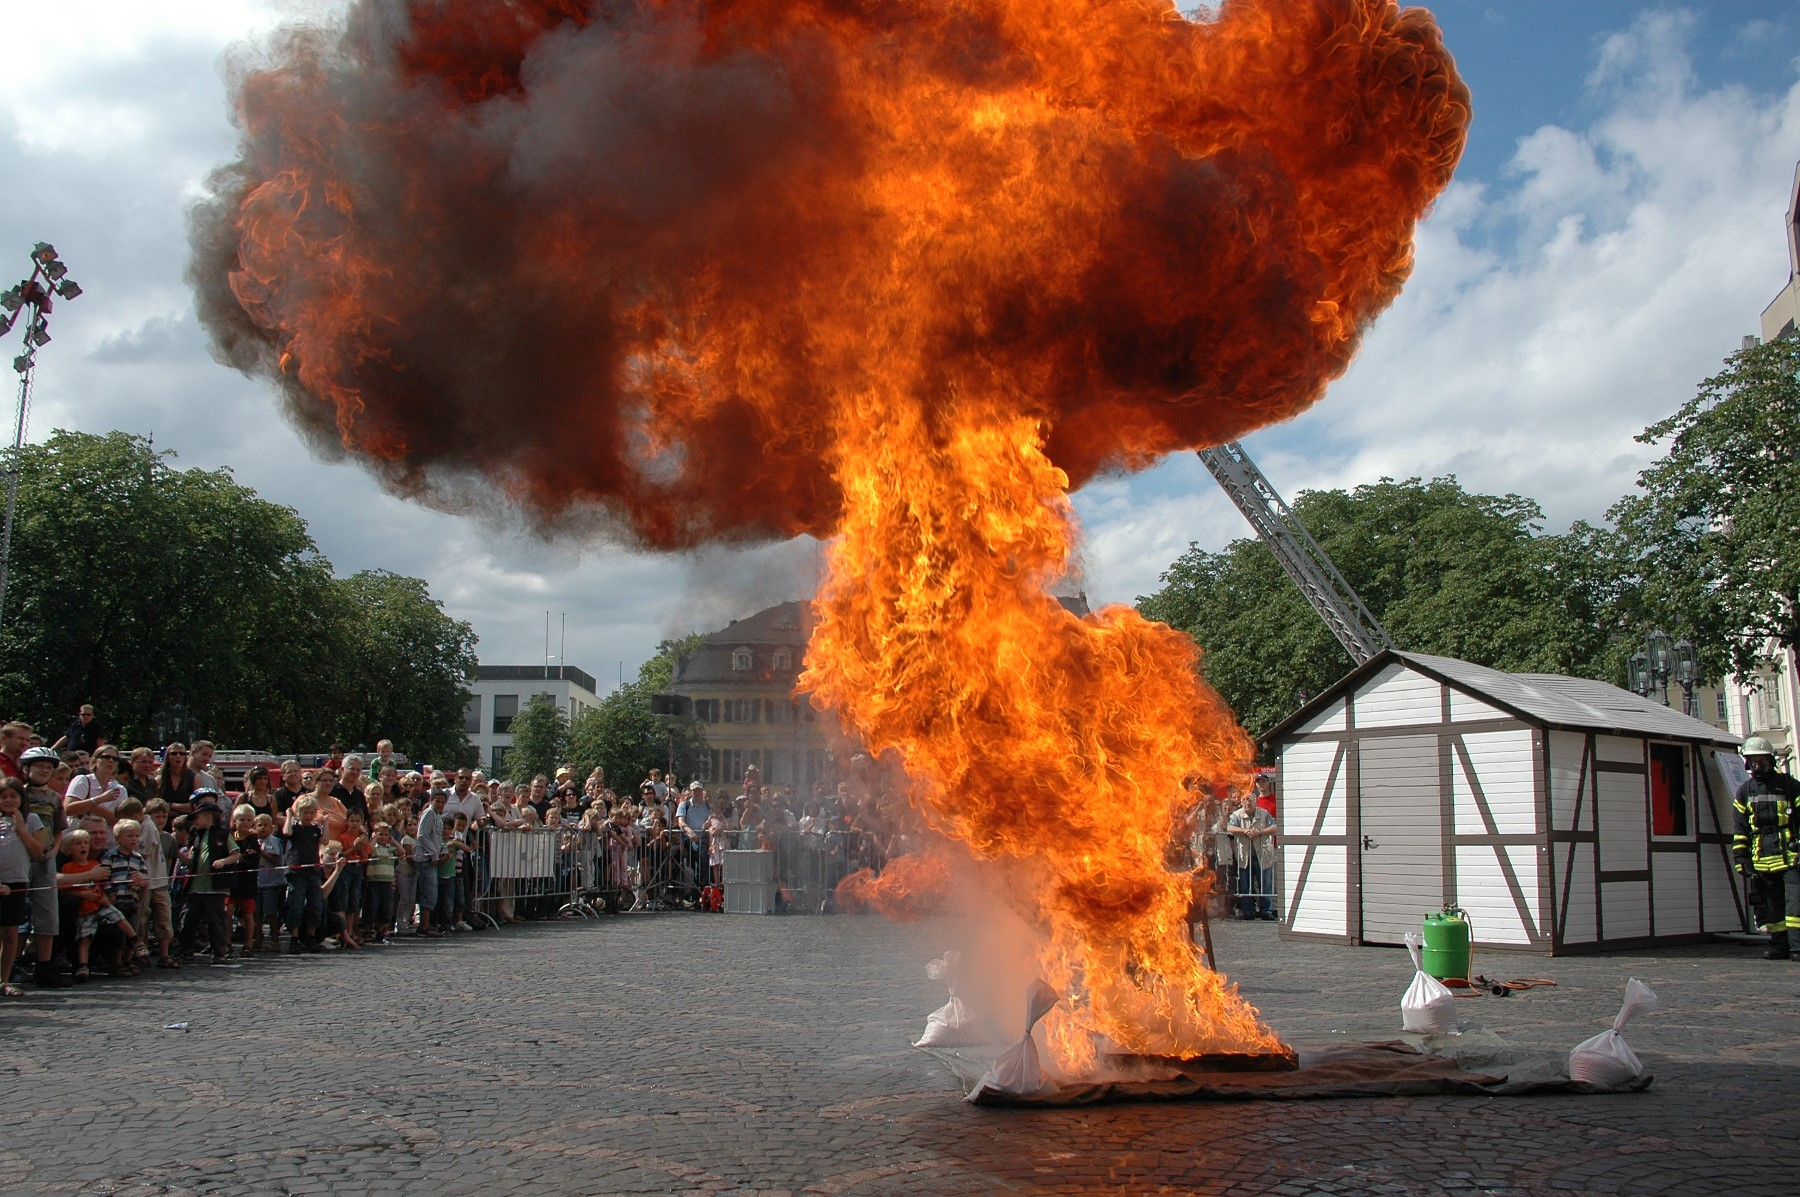
\includegraphics[width=0.89\textwidth]{Grafiken/Basics/Fire/Fettbrand.jpg}
	\centering
	\begin{footnotesize}
		\caption{Fettbrand. Flammen und Rauch mischen sich bei expolosionsartigem Feuer. \\Bild: Der Sascha(\url{https://commons.wikimedia.org/wiki/File:TDFw_135a.jpg}), „TDFw 135a“, \url{https://creativecommons.org/licenses/by-sa/3.0/legalcode}  }

		\label{fig:fettbrand}
	\end{footnotesize}
\end{figure}

<<<<TODO>>>>

\subsubsection{Rauch}
<<<<TODO>>>>

\subsubsection{Partikelsysteme}
<<<<TODO>>>>

\subsection{Texture Mapping}

Texture Mapping bezeichnet ein Verfahren, welches zweidimensionale Texturen auf ein dreidimensionales Objekt
abbildet. Um die flachen Texturen auf die Oberfläche des Meshs abbilden zu können, muss das Objekt 'UV-unwrapped' werden.
Durch diesen Vorgang wird jedem Punkt auf der Oberfläche des Meshs ein Punkt auf der Textur zugewiesen \parencite{Catmull1974} \parencite{Blinn1976}.
Ein sehr einfaches Beispiel zur Veranschaulichung ist dabei das Würfelnetz (\autoref{fig:wuerfelnetz}).
\begin{figure}[h]
	\centering
	\includegraphics[width=0.69\textwidth]{Grafiken/Basics/Mapping/Würfelnetz.png}
	\begin{footnotesize}
		\caption{Würfelnetz.}
		\label{fig:wuerfelnetz}
	\end{footnotesize}
\end{figure}

Texture Mapping sorgt dafür, die Objekte 'anzumalen'.
Reale Objekte haben oft sehr detaillierte Oberflächeneigenschaften und sind eigentlich niemals wirklich glatt.
Geometrische Unebenheiten und Feinheiten, wie Kratzer, Rillen und Schmutz lassen sich zwar durch 
Farbtexturen andeuten, jedoch bleibt die Oberfläche komplett glatt. Diese rauhen Oberflächen zu modellieren resultiert
aber in einer deutlich höheren Polygon-Anzahl, was die Performance in großen Szenen schnell negativ beeinflussen kann.
Daher wurden Mapping-Verfahren als Ergänzung entwickelt, um die virtuelle Auflösung
solch komplexer Oberflächen kostengünstig zu erhöhen, ohne dabei die Komplexität der Geometrie zu verändern.
Dabei gibt es verschiedenste Shader, welche unter Anwendugn weiterer, spezieller Texturen eine deutlich detailliertere
Oberfläche simulieren können.


% \subsubsection{Normal Mapping}
\subsubsection{Bump Mapping}

Eine Möglichkeit, mit der sich die Oberflächen mit mehr Details rendern lassen, ist das Rendering
mithilfe von sogenannten Bump Maps.
Hierbei werden auf Basis von Texturen, welche zusätzliche Informationen zu den Oberflächen enthalten,
Details generiert, welche den Eindruck einer realistischen Struktur der Oberfläche erzeugen.
Dabei ist es nicht notwendig, dass die Geometrie an sich Informationen dazu beinhaltet \parencite{Blinn1978}.

Bump Maps sind Texturen, basierend auf Graustufen, bei denen die Helligkeit eines Pixels
einen Höhenwert repräsentiert. Schwarz steht mit dem Wert 0 für den tiefsten Punkt, und weiß mit dem Wert 1 für den höchsten Punkt.
Eine verbesserte Variante der Bump Maps sind die Normal Maps.
Hier werden die Richtungen der Normalen in jedem Pixel durch einen Vektor repräsentiert,
welcher sich aus den RGB-Werten eines jeden Pixels ergibt. Daraus lassen sich Schattierungen simulieren,
welche kleine Unebenheiten (mit geringer Tiefe) wie Beulen oder Kratzer realistischer aussehen lassen.
Dieser wird aus Lichtquellen, deren Einfallsrichtung und den Normalen aus der Textur berechnet.
Somit wird auch bei geringer Polygonanzahl eine deutlich realistischer aussehende Oberfläche gerendert.
\parencite{Cohen1998}.

Diese Texturen bieten einen sehr kostengünstigen
Ansatz, um Tiefe zu simulieren. Shaderberechnungen, basierend auf diesen Methoden, sind dabei aber nicht abhängig
vom Betrachtungswinkel und sehen schnell unnatürlich verzerrt aus.
Von vorne betrachtet funktioniert die Illusion. Je spitzer jedoch der Winkel zwischen Betrachter und
Oberfläche wird, desto auffälliger wird die Tatsache, dass die Silhouette des Objekts immer
noch flach ist, da die Geometrie hierbei nicht verändert wird.
Zusätzlich wird die Effektivität von reinem Normal Mapping in VR-Umgebungen aufgrund der Unabhängigkeit vom Betrachtungswinkel
geschwächt. 

\begin{figure}[h!t]
	\centering
	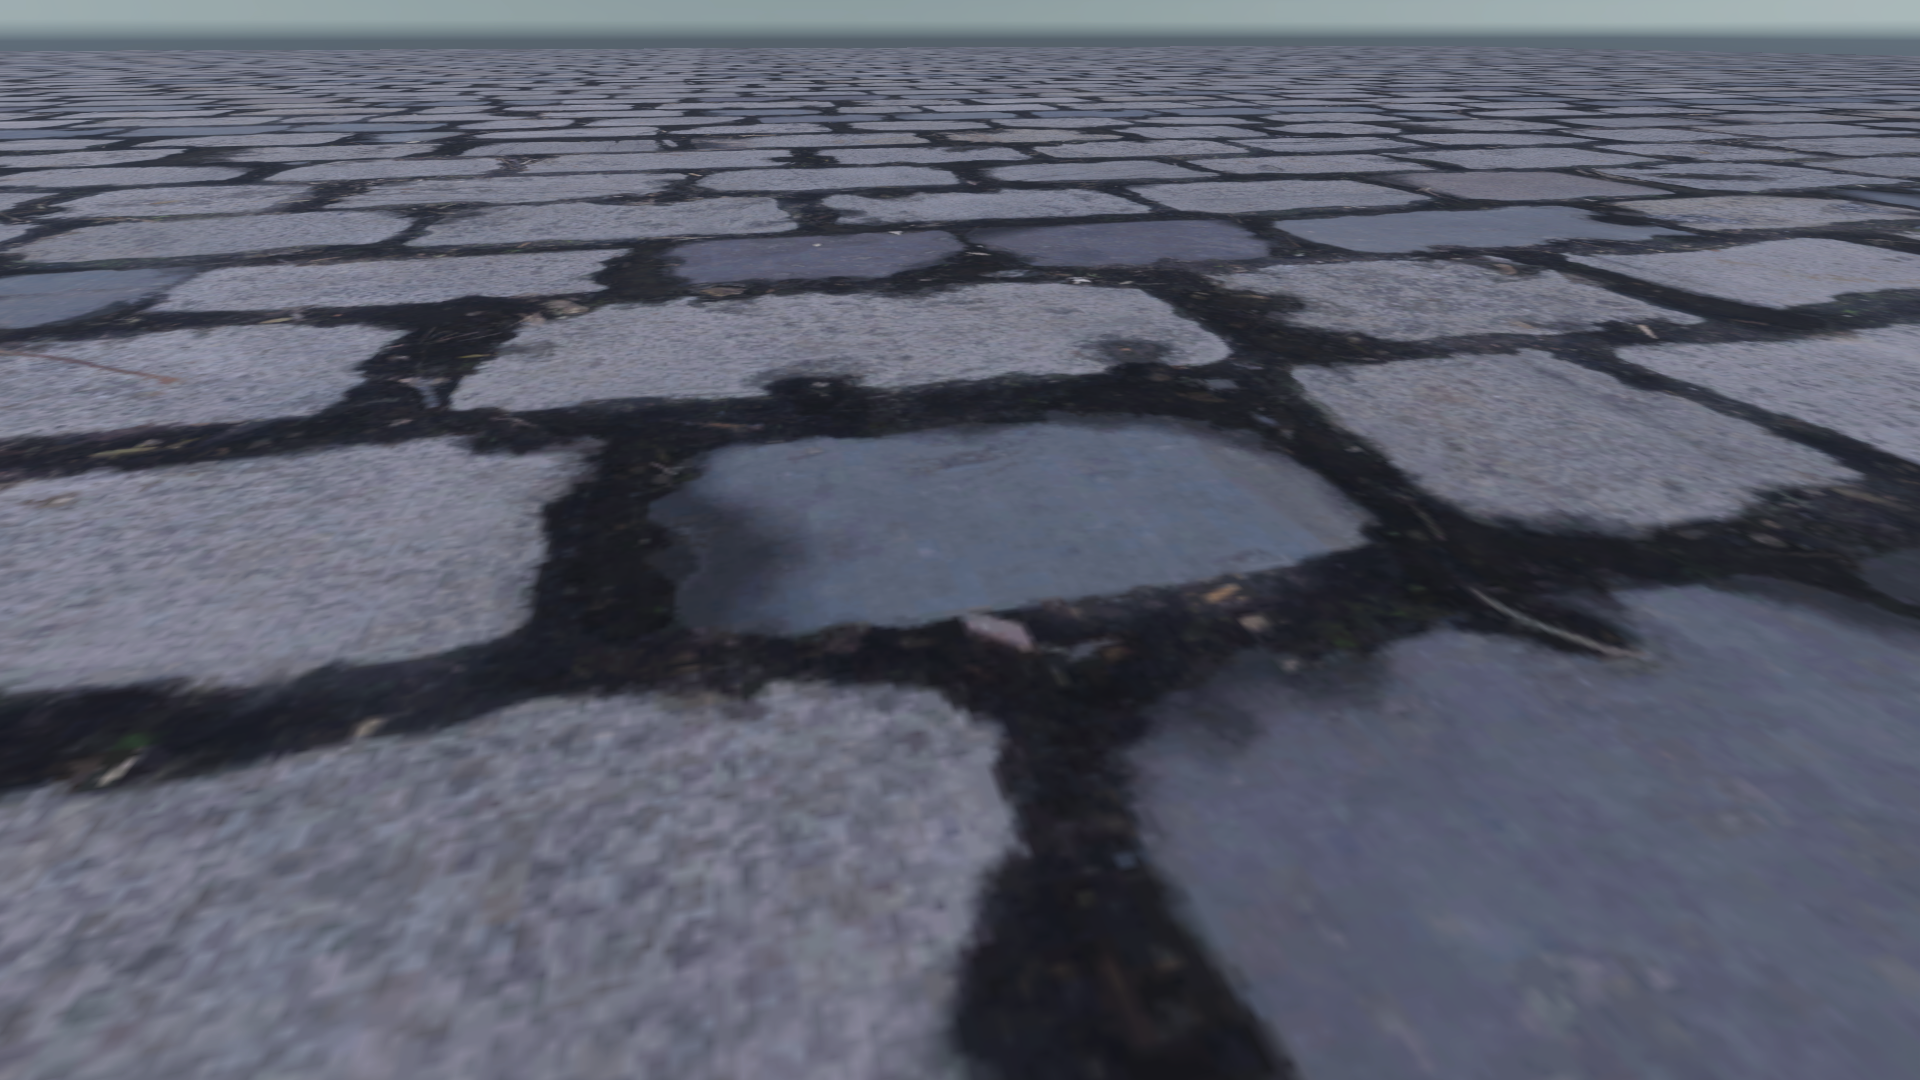
\includegraphics[width=0.49\textwidth]{Grafiken/Basics/Mapping/Vergleich_Diffuse.png}
	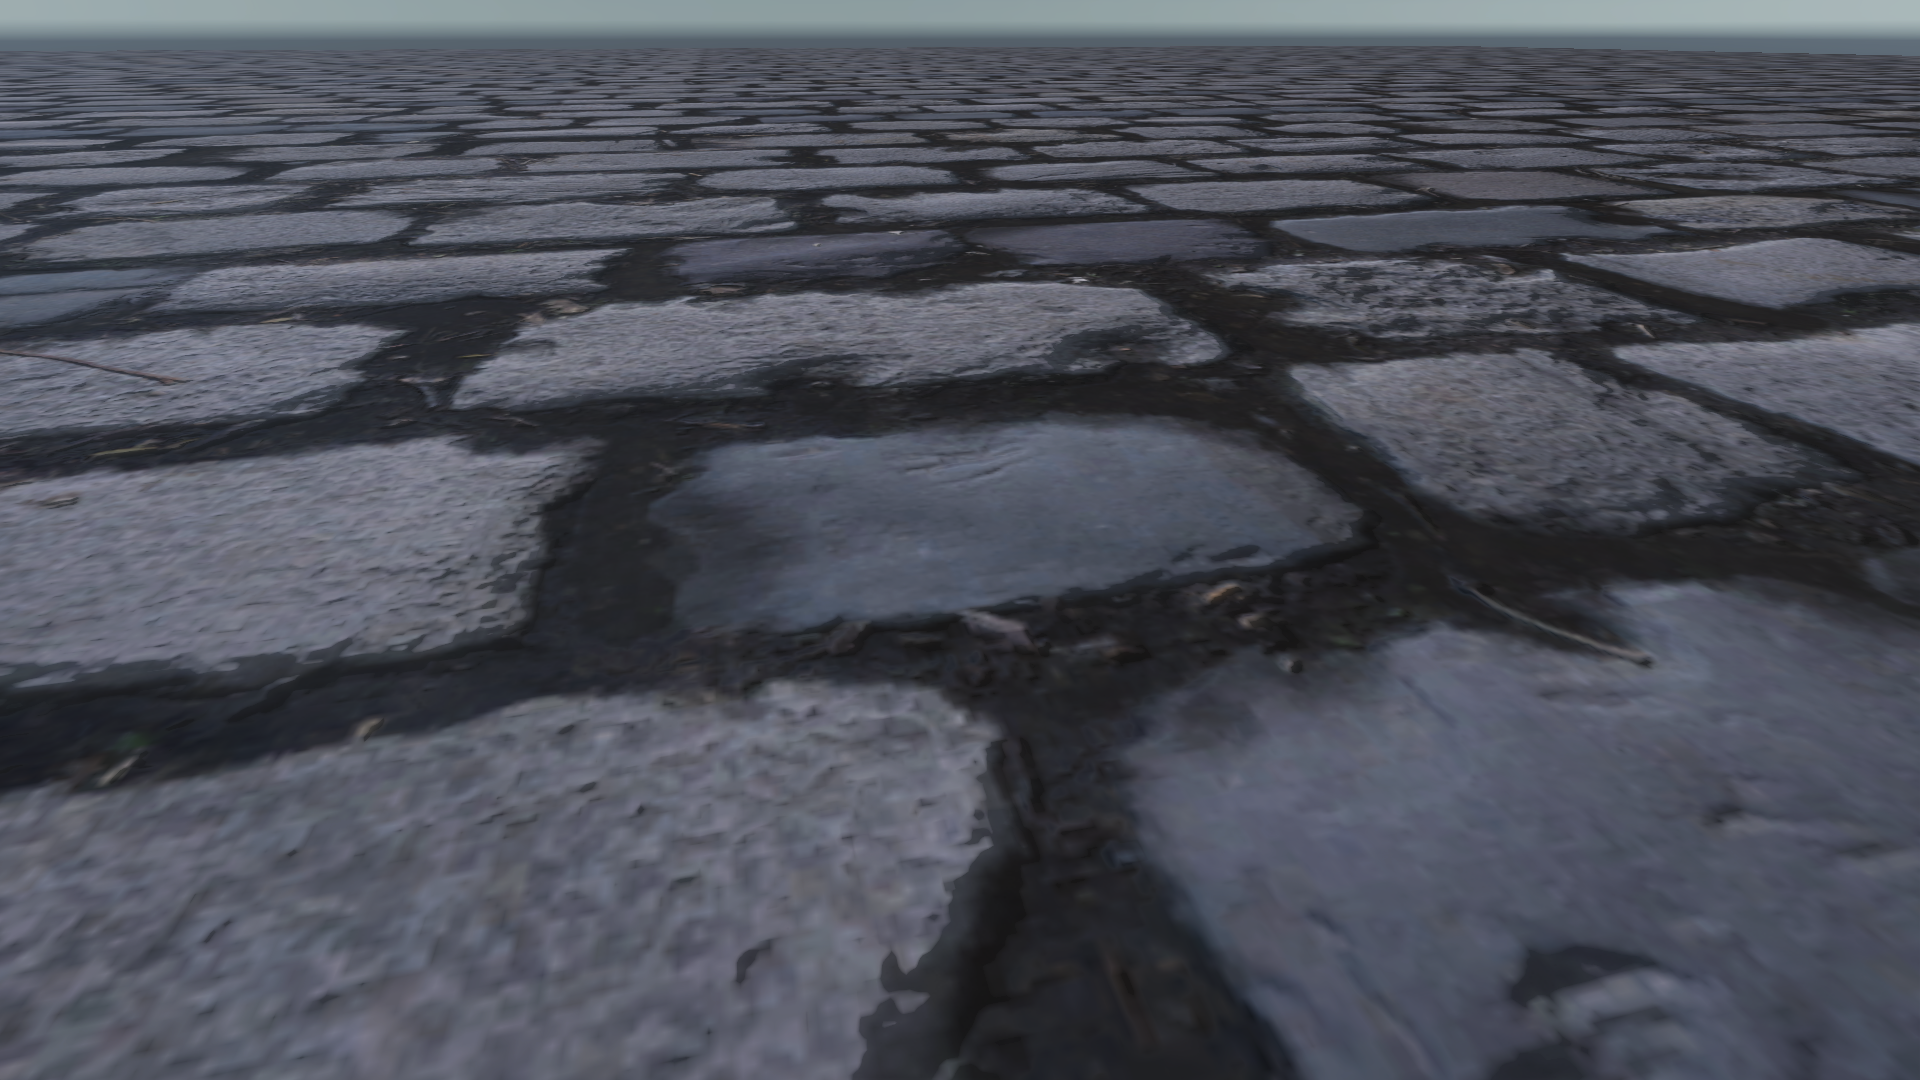
\includegraphics[width=0.49\textwidth]{Grafiken/Basics/Mapping/Vergleich_Normal.png}
	\begin{footnotesize}
		\caption{links: Einfache diffuse Beleuchtung der Textur, rechts: Normal Mapping. Beide Geometrien sind komplett flach. 
		Hierbei sieht man gut den Unterschied zwischen dem flachen Look
		der diffus beleuchteten Textur und dem realistischeren Aussehen durch Einbeziehen der Oberflächennormalen aus der Normal Map.}
	\end{footnotesize}
\end{figure}

\subsubsection{Displacement Mapping}
Mit Displacement Mapping werden dagegen tatsächlich, mithilfe von Heightmaps, die Positionen
der Vertices entlang ihrer Normalen versetzt \parencite{Cook1984,Cook1987}. Dadurch kommt es nicht zu blickwinkelabhängigen Artefakten
und die Illusion von Tiefe wird real. Objekte sehen aus einem flachen Winkel betrachtet nicht mehr
glatt aus, sondern haben tatsächlich Struktur in ihrer Oberfläche. Damit dieser Effekt jedoch zustande kommt,
muss das Mesh in einer gewissen Auflösung zur Verfügung stehen. Je nach Detailreichtum der Heightmap
muss die Geometrie dabei in weitere Polygone unterteilt werden. Der Vorteil hierbei ist der hohe
Grad an Realismus. Ein deutlicher Nachteil liegt dabei allerdings in der Performance.
Ein weitgehender Einsatz von Displacement Mapping kann eine hohe Polygonanzahl schnell
negativen Einfluss auf die Renderingzeiten nehmen. 


\subsubsection{Parallax Mapping}

Parallax Mapping (oder auch Offset (Bump-)Mapping) ist eine weitere Methode, um sich die Möglichkeiten von
Bump Mapping-Verfahren zunutze zu machen. Anders als bei tatsächlicher Modifizierung der Vertices
durch Displacement Maps werden hier nur die Texturkoordinaten abhängig vom Blickwinkel verschoben. \parencite{Kaneko2001, Welsh2004}
Durch Bewegung der Oberfläche oder des Betrachters entsteht somit ein realistischerer Eindruck
von Tiefe in der Textur, welcher den des Displacement Mappings approximiert darstellt.
Dabei ist Parallax Mapping allerdings immer noch deutlich effizienter als echtes Vertex-Displacement
und eignet sich daher eher für Echtzeitrenderings.
Parallax Mapping alleine simuliert zwar den Parallax-Effekt, jedoch ist es hiermit nicht möglich, die Silhoutte zu verändern und
Selbstschattierung oder -verdeckung vorzutäuschen.


\subsubsection{Parallax Occlusion Mapping}
\label{sec:3.3.4}

\begin{figure}[h]
	\centering
	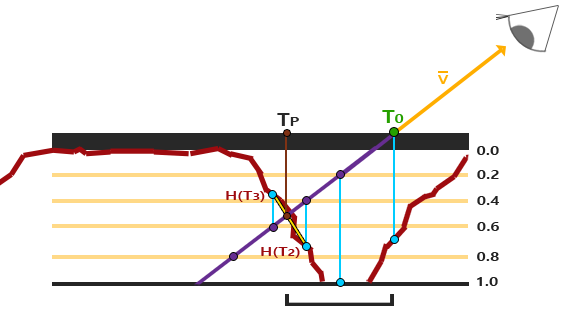
\includegraphics[width=0.8\textwidth]{Grafiken/Basics/Mapping/Infografik_POM.png}
	\begin{footnotesize}
		\caption{Verschiebung der Texturkoordinaten beim Parllax Occlusion Mapping}
	\end{footnotesize}
\end{figure}


Parallax Occlusion Mapping (POM) ist eine komplexere, verbesserte Variante des Parallax Mapping, basierend auf einem Per-Pixel Ray Tracing.
Das Ziel ist auch hier wieder das Vorherige: Detaillierte Oberflächen ohne den Preis von teuren Vertexverschiebungen.
Diese Details lassen sich abhängig vom Blickwinkel aus jeder Perspektive korrekt darstellen.
Durch Einsatz von dynamischer Beleuchtung und Selbstokklusion kann außerdem eine korrekte Selbstschattierung simuliert werden \parencite{Brawley2004, Tatarchuk2006}.
Die Informationen aus der Heightmap werden hierbei für Berechnungen im Fragmentshader verwendet.
Anstatt wie beim Displacement Mapping Details zu extrudieren, wird bei POM in die Tiefe simuliert.
Hierbei wird für die Oberfläche der Wert 1.0, und damit der höchste Punkt, angenommen.
Zunächst wird für jeden zu rendernden Pixel mittels Ray Castings vom Betrachter zur Geometrie-Oberfläche ein Schnittpunkt  $T_0$ ausfindig gemacht.
Der Strahl $\vec{v}$ wird nun weiter durch das – durch die Heightmap ausgedrückte – Volumen verfolgt und Schrittweise abgetastet. Wenn sich der Strahl 
mit der Heightmap im Punkt $T_P$ schneidet, kann mit der Position die neue, zu rendernde Texturkoordinate ermittelt werden. 
Je geringer die Schrittweite ist, desto genauer kann die Oberfläche gerendert werden.
Ist die Schrittgröße zu groß, kann die Heightmap nicht detailliert genug abgetastet werden und es entstehen Aliaseffekte. Es zeichnet sich
ein Treppeneffekt ab (\autoref{fig:alias}). Zusätzlich kann ein zu starkes Offset die Textur unnatürlich weit verzerren. 


\begin{figure}[ht]
	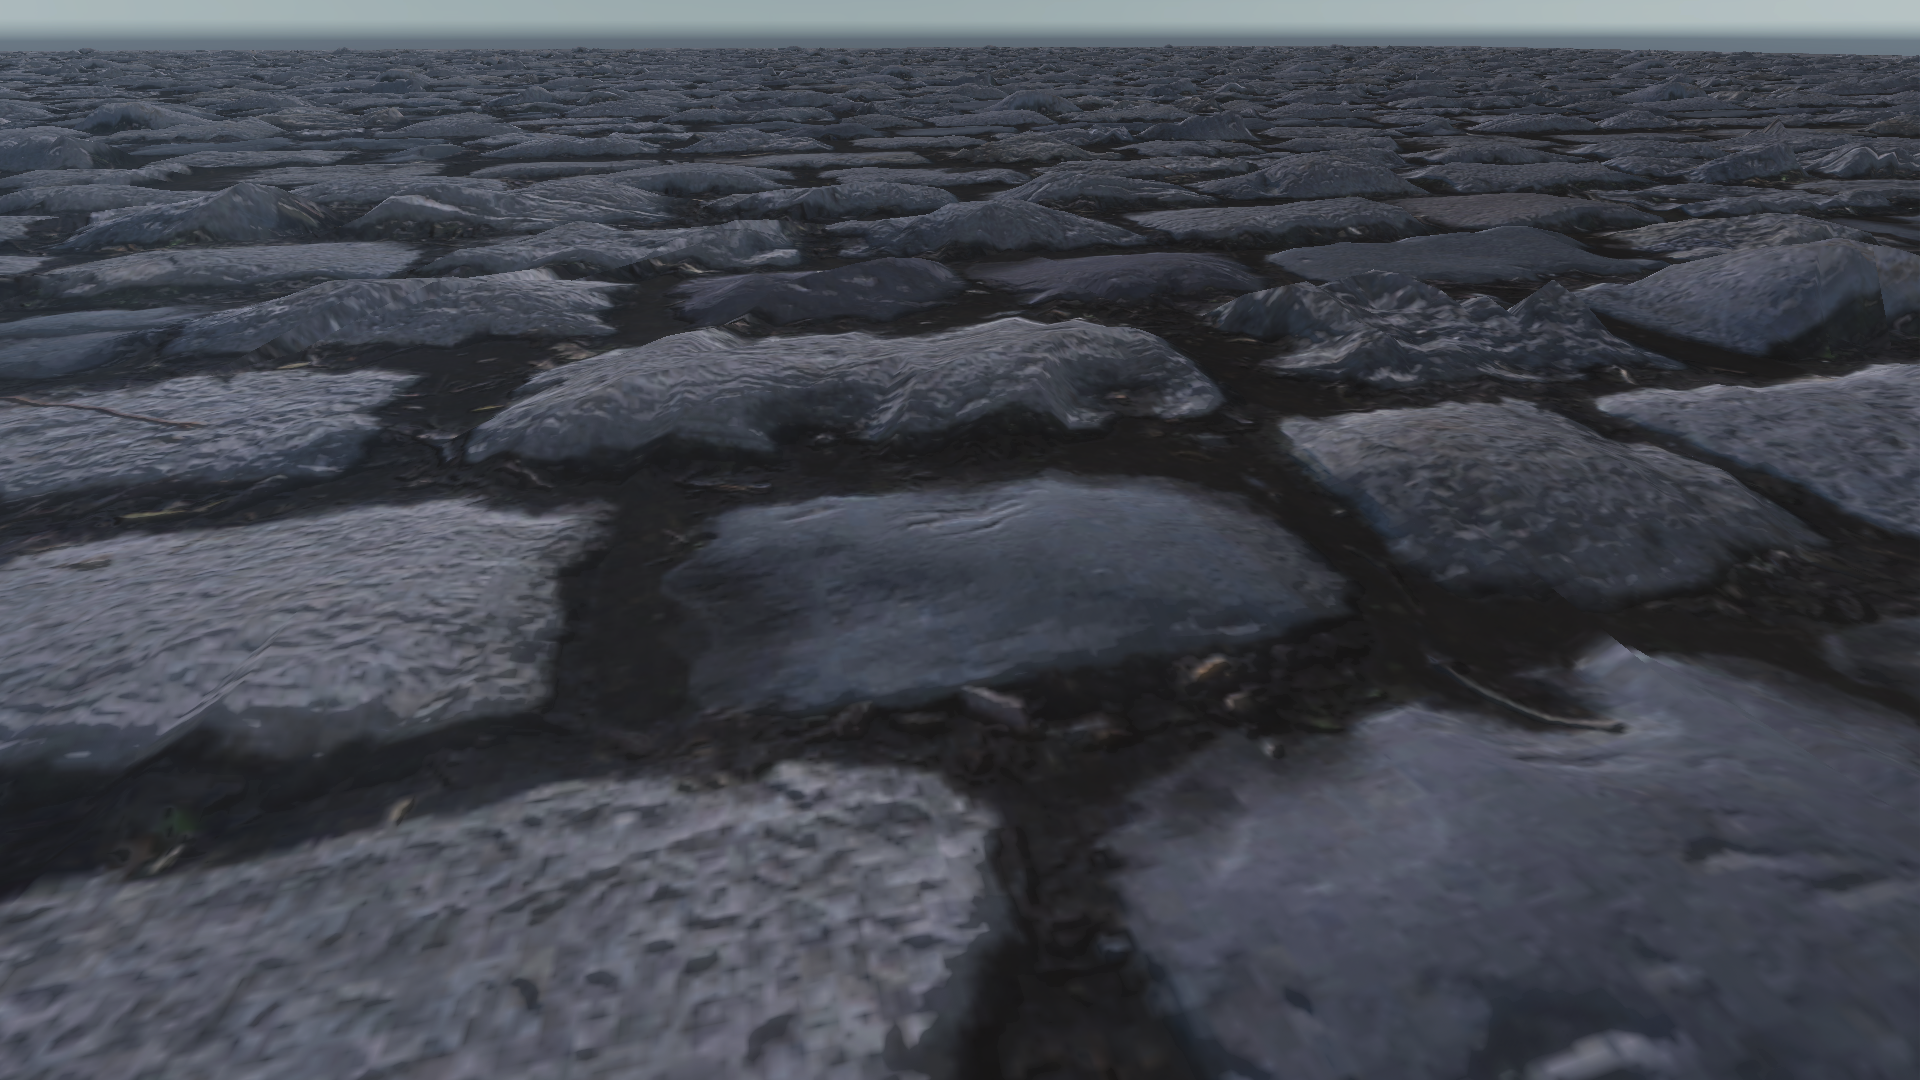
\includegraphics[width=0.49\textwidth]{Grafiken/Basics/Mapping/Vergleich_DisplacementNormalTesselated.png}
	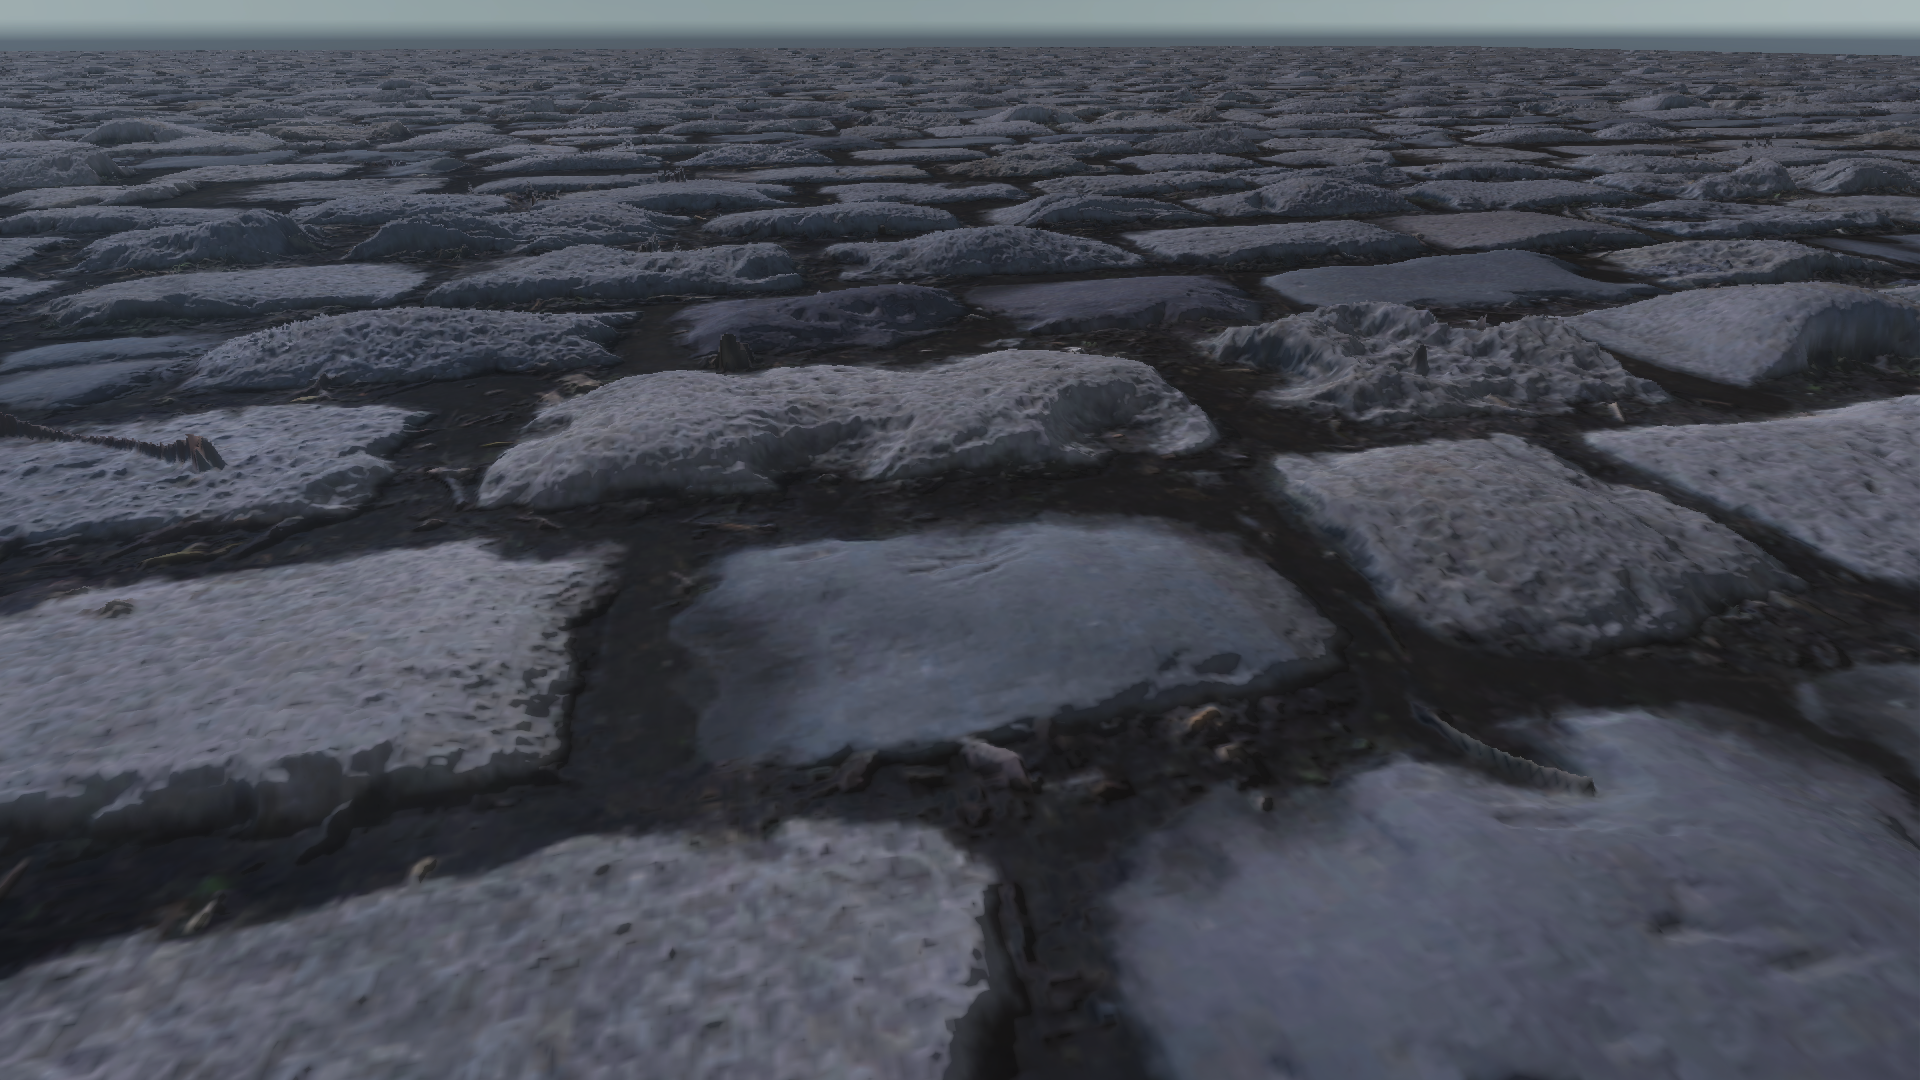
\includegraphics[width=0.49\textwidth]{Grafiken/Basics/Mapping/Vergleich_POM_64Steps.png}
	\begin{footnotesize}
		\caption{links: Displacement Map, Normal Map und 50-facher Tesselation, rechts: Parallax Occlusion Mapping mit 64 Samples. 
		Beide Methoden sehen sich sehr ähnlich, der Unterschied ist jedoch, dass für die Displacement Map-Methode in diesem Beispiel die 50-fache Anzahl an
		Dreiecken gebraucht wird.}
	\end{footnotesize}
\end{figure}


\begin{figure}[h]
	\centering
	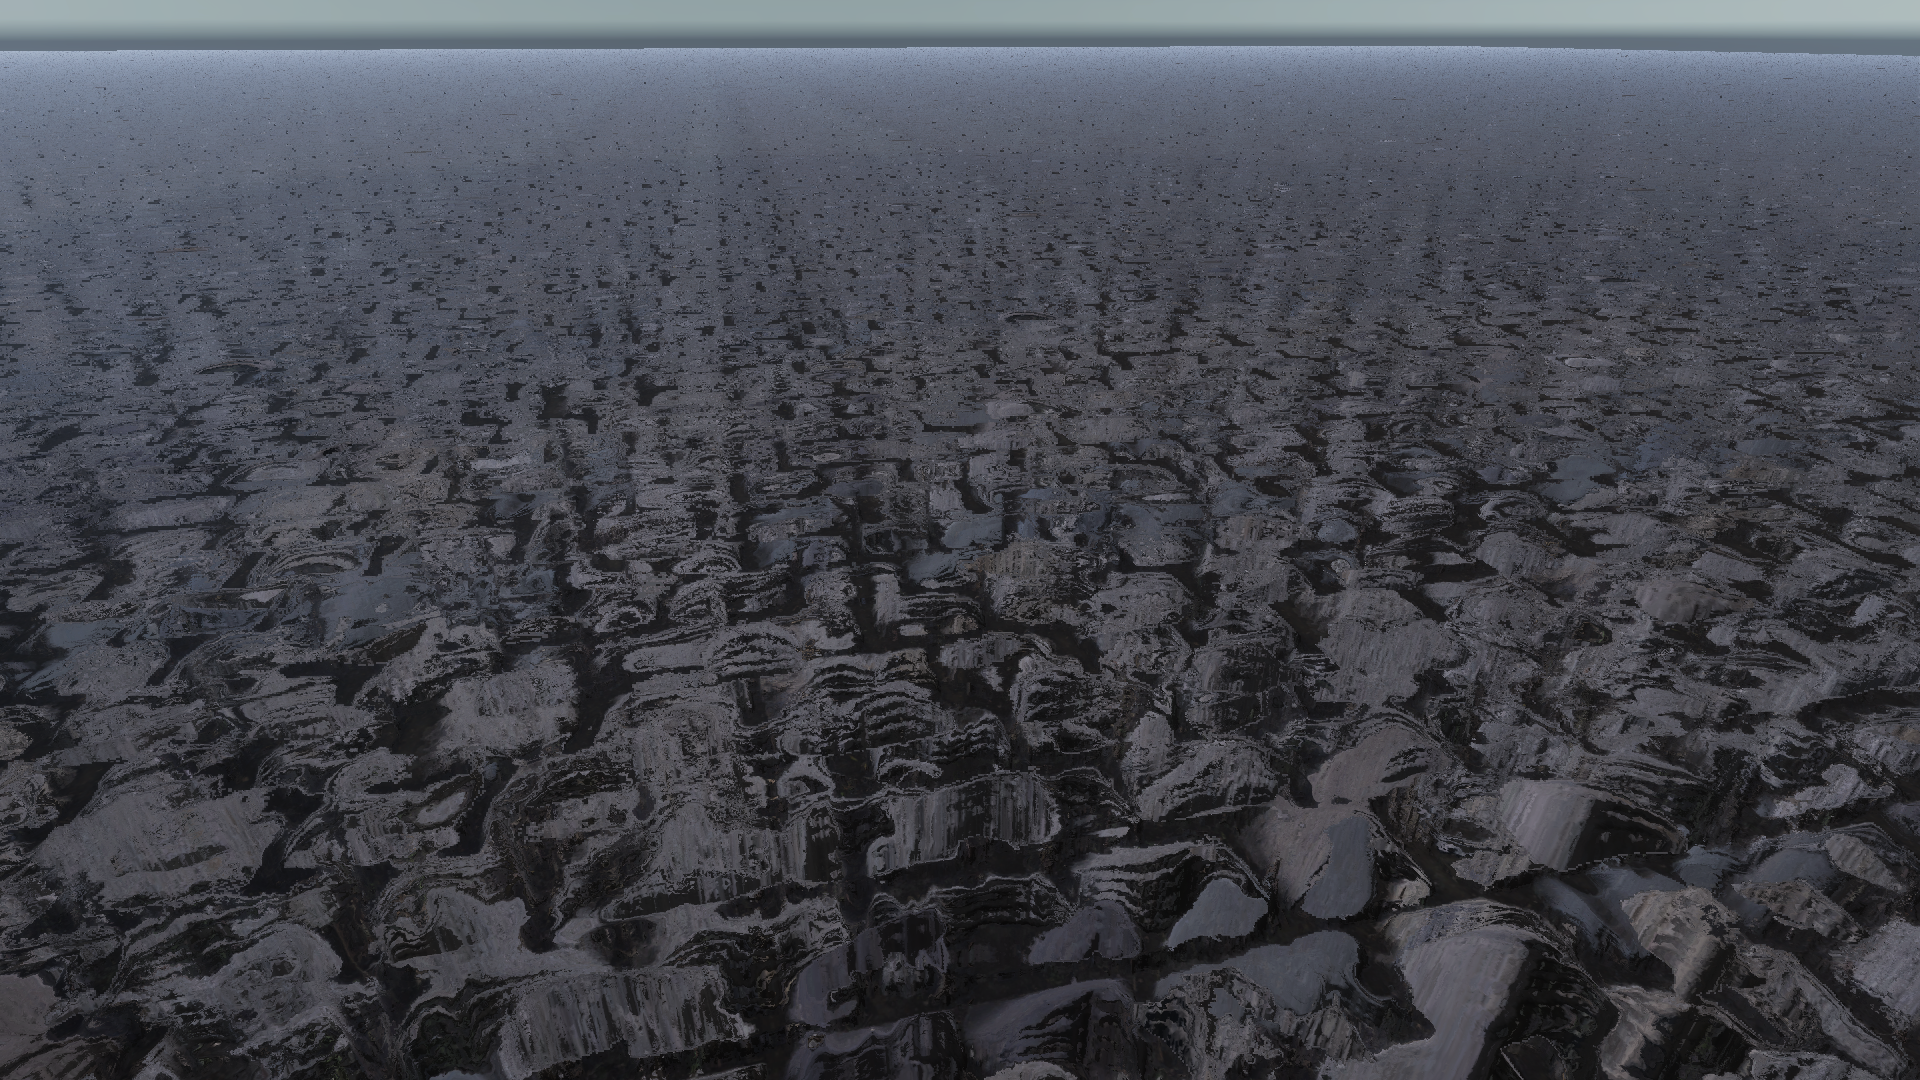
\includegraphics[width=1\textwidth]{Grafiken/Basics/Mapping/aliasing.png}
	\begin{footnotesize}
		\caption{Aliasingeffekt bei zu geringer Sampleanzahl mit 4 Schritten.}
		\label{fig:alias}
	\end{footnotesize}
\end{figure}

\subsection{Volume Rendering}

Unter dem Begriff Volume Rendering versteht sich eine Reihe von Methoden, die es ermöglichen, ein 3D-Datenset zu visualisieren.
Anders als beim Rendern von Geometrien mit einer festen Oberfläche, geht es hierbei darum, alle Daten aus
dem jeweiligen Volumen darstellen zu können. Dies sind beispielsweise volumetrische Effekte wie Feuer und Rauch, Wolken oder Nebel,
welche sich, aufgrund ihrer gasförmigen Eigenschaften, nicht wirklich realistisch mit Geometrie darstellen lassen.
Volumen haben keine wirkliche Oberfläche, sondern bestehen aus unzähligen winzigen Partikeln oder Gasen.
Möchte man also solche Volumen darstellen, so geraten die bisherigen Herangehensweisen, die sich die Oberflächen der Objekte zunutze machen,
schnell an ihre Grenzen. Beim Grundgedanken des Volume Renderings geht es daher um die Frage, wie das Licht durch diese Volumen
wandert und welchen Einfluss die Partikel darauf haben.
Es gibt einige Faktoren, die beeinflussen können wie das Licht verändert wird bis es das das Auge nach Austritt aus einem Volumen erreicht.
Während das Licht durch solch ein Volumen wandert, kann es absorbiert, reflektiert oder gestreut werden.
Die Abschwächung durch Streuung und Absorption des Lichtes beim Durchlaufen eines Volumens kann vereinfacht mithilfe des Lambert-beerschen Gesetzes wie in \autoref{eqn:beer}
approximiert werden \parencite{Mayerhofer2020}.
Der Absorptionskoeffizient $\sigma_a$ beschreibt dabei die Wahrscheinlichkeit, dass ein Photon auf der Strecke $d$ durch das Medium absorbiert oder anderweitig
reflektiert wird.

\vspace{-0.5cm  }
\begin{equation}
	\label{eqn:beer}
	I_{out} = I_{in} \cdot e^{- ( d \cdot\sigma_a  )}.
\end{equation}





\subsubsection{Ray Marching}

Ray Marching ist eine dieser Möglichkeiten, ein Volumen darzustellen. Die Idee hierbei ist es – ähnlich wie beim Ray Tracing –
Strahlen von der Kamera aus durch jeden Pixel des zu rendernden Bildes zu schicken und dabei in festgelegten Abständen zu prüfen,
ob der Strahl auf etwas trifft.
Der Unterschied besteht hierbei jedoch darin, dass sich Ray Marching auf sogenannte '\textit{signed distance functions}' (SDF) bezieht.
Mit SDFs lässt sich beschreiben, wie weit die nächstgelegene Oberfläche entfernt ist. Dazu wird die Entfernung zu jedem Objekt
in der Szene berechnet und die kürzeste Distanz gewählt.

\begin{figure}[h]
	\centering
	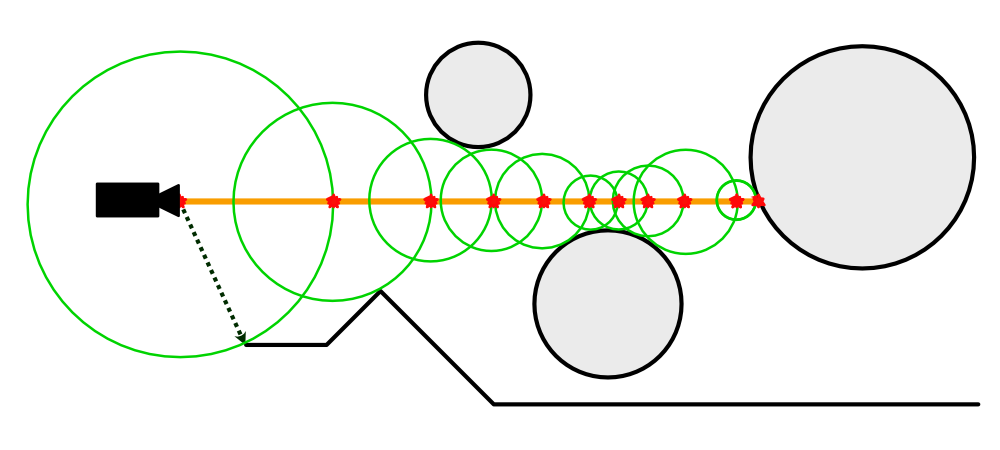
\includegraphics[width=0.80\textwidth]{Grafiken/Basics/Volume/Sphere_Tracing.png}
	\begin{footnotesize}
		\caption{Sphere Tracing: Der Algorithmus wird so lange wiederholt, bis der Radius/Abstand zum nächstgelegenen
			Objekt unter einen bestimmten Grenzwert fällt.}
	\end{footnotesize}
\end{figure}


Im ersten Schritt muss also die Distanz zur nächstgelegenen Oberfläche gefunden werden. Daraus ergibt sich ein Radius, in dem sich
mit Sicherheit nichts anderes befindet. Der Strahl bewegt sich nun um die Länge des berechneten Radius in seine vorgesehene Richtung.
Anschließend werden diese beiden ersten Schritte an der neuen Position wiederholt. Dies passiert so lange, bis die Entfernung gegen einen festgelegten
Grenzwert läuft. Dies deutet darauf hin, dass eine Oberfläche getroffen wurde. Diese Variante von Ray Marching wird auch
'\textit{Sphere Tracing}' genannt \parencite{Hart96}. Sphere Tracing ist, im Gegensatz zu einer konstanten Schrittweite, ein effizienter Algorithmus,
um Oberflächen entlang des Strahls zu finden, da hiermit die Anzahl der benötigten Schritte deutlich reduziert werden kann.

Jede Oberfläche einer Szene kann durch eine solche Distanzfunktion dargestellt werden.
Eine Kugel lässt sich also beispielsweise durch die folgende Funktion mit ihrer Position in Weltkoordinaten und einem Radius darstellen:

\vspace{0.5cm}
\begin{lstlisting}[language={[Sharp]C}, label={lst:sphereSDF}, caption={SDF einer Kugel im Ursprung},captionpos=b, frame=single]
float sdfSphere( vec3 pos, float radius ){
	return length(pos)-radius;
}
\end{lstlisting}

Mithilfe dieser Funktionen lassen sich mehrere SDFs auf verschiedene Art und Weise kombinieren und deformieren, wodurch sich neue Formen
erzeugen lassen (\textbf{\autoref{fig:sdfOperators}}).
Dabei gibt es verschiedene Möglichkeiten, wie z.B. die Vereinigung zweier Objekte, die Schnittmenge oder auch die Differenz.
Mit dem Smooth Union-Operator lassen sich beispielsweise sogenannte Blobs oder Metaballs erzeugen, indem zwischen
den Oberflächen interpoliert wird, sodass diese Geometrien den Anschein erwecken, miteinander zu verschmelzen.

\begin{figure}[h]
	\centering
	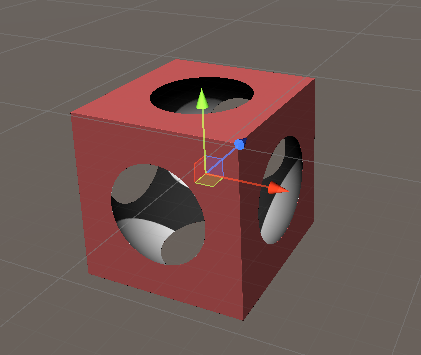
\includegraphics[height=0.15\textheight]{Grafiken/Basics/Volume/sdf_cut.png}
	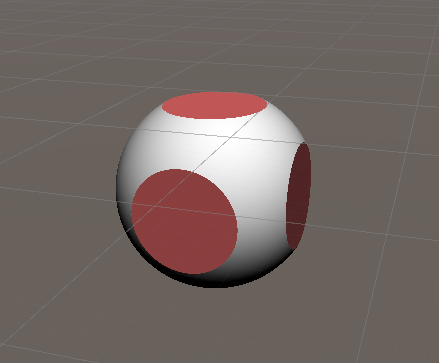
\includegraphics[height=0.15\textheight]{Grafiken/Basics/Volume/sdf_mask.png}
	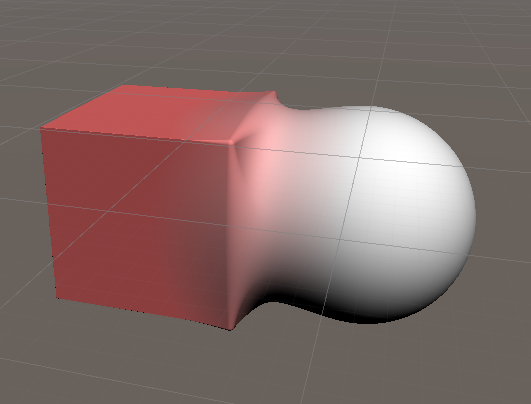
\includegraphics[height=0.15\textheight]{Grafiken/Basics/Volume/sdf_union.png}
	\begin{footnotesize}
		\caption{Beispiele von verschiedenen SDF-Operatoren.
			Von links: Subtraction, Intersection, Smooth Union.}
		\label{fig:sdfOperators}
	\end{footnotesize}
\end{figure}




\subsubsection{Volume Ray Marching}

\begin{figure}[h]
	\centering
	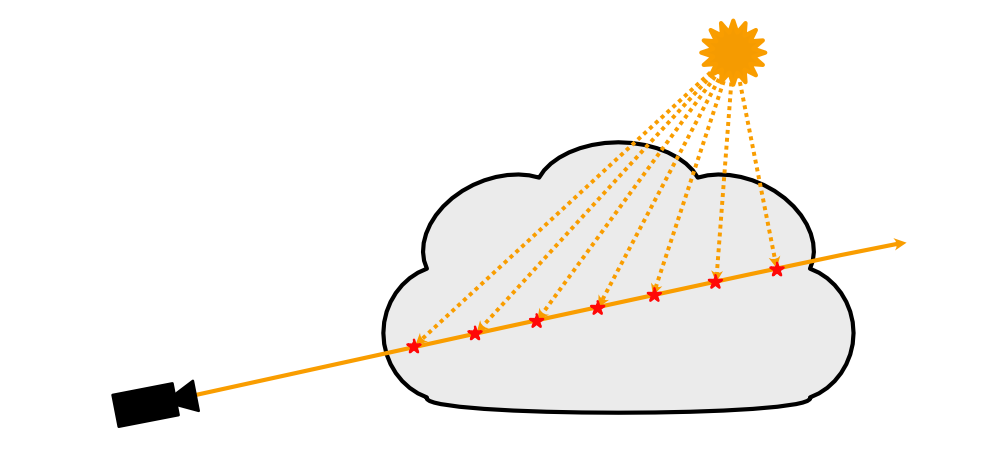
\includegraphics[width=0.80\textwidth]{Grafiken/Basics/Volume/Volume_RayMarching.png}
	\begin{footnotesize}
		\caption{Vereinfachte Darstellung des Volume Ray Marching. Der Weg des Lichtes durch
			das Medium. In der Realität ist die Berechnung aufgrund von In- und Out-Scattering, Absorption oder Emissionen innerhalb des
			Volumens komplexer.}
		\label{fig:volumeRayMarching}
	\end{footnotesize}
\end{figure}


Möchte man nun aber komplexere Volumen darstellen, so gelingt dies unter Einsatz einer Volumentextur. Der Ansatz bleibt dabei der Gleiche.
Es wird ein Objekt benötigt, welches als Volumen Container fungiert. Dieses kann in Form von oben beschriebenen SDFs repräsentiert sein.
Innerhalb dieser Geometrie kann nun alles mögliche dargestellt werden, da hierbei keine feste Oberfläche die Grundlage des
Volumens darstellt. Es lässt sich mittels Code beispielsweise innerhalb eines Würfels eine Kugel darstellen (\textbf{\autoref{fig:sphereInsideCube}}).

\begin{figure}[h]
	\centering
	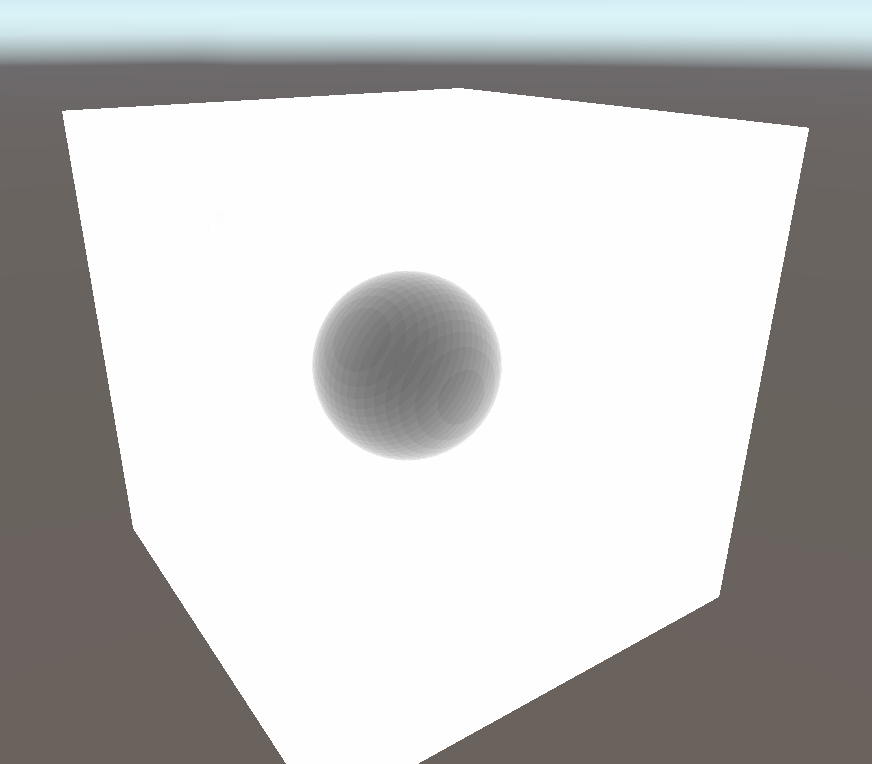
\includegraphics[width=0.80\textwidth]{Grafiken/Implementation/Raymarch/sphereInsideCube.png}
	\begin{footnotesize}
		\caption{Kugel im Inneren einer Box mittels Ray Marching gerendert.}
		\label{fig:sphereInsideCube}
	\end{footnotesize}
\end{figure}


Wurde per Sphere Tracing eine Oberfläche ermittelt, so wird in festgelegten Schritten (sample rate) das Innere der Geometrie durchlaufen
und an jedem Schritt ein Wert berechnet, der sich aus Farbe, Dichte und Tiefe im Volumen ergibt (\textbf{\autoref{fig:volumeRayMarching}}).
Mithilfe von \autoref{eqn:drebin} \parencite{Drebin1988} lässt sich durch das aus einem Voxel austretende Licht ein Farbwert bestimmen.
Voxel sind das Äquivalent zu einem Pixel im dreidimensionalen Raum und werden durch ein 3D-Gitternetz repräsentiert.

\begin{equation}
	\label{eqn:drebin}
	C_{out} = C_{in} \cdot (1 - O(x)) + C(x) * O(x).
\end{equation}
(Berechnung der Farbe des austretenden Lichts mit $O(x)$ als Opacity und $C(x)$ als Farbe des Voxels.)


<<<<Formel stimmt nicht ganz, muss ich noch mal recherchieren>>>>

\textit{
	Ein Nebenprodukt, das sich durch Ray Marching ergibt, ist eine Variante des Ambient Occlusion \parencite{Evans2006}.
}
→ Näher beschreiben oder weglassen



